\documentclass[class=report, crop=false, 12pt,a4paper]{standalone}
\usepackage{enumitem}
\usepackage{multicol}
\usepackage{graphicx}
\usepackage{float}
\usepackage{amsmath}
\usepackage{amssymb}
\usepackage{mathtools}
\usepackage{siunitx}
\usepackage{commath}
\usepackage{array}
\usepackage{natbib}
\usepackage[a4paper,width=150mm,top=25mm,bottom=25mm]{geometry}
\setlength{\parindent}{0pt}
\begin{document}
\section{Plane stress state}
\subsection{State of equilibrium}
The basis of structural analysis is the \textbf{equilibrium state}:
\begin{quotation}
    If a configuration is in equilibrium, the resultant of all external forces and moments is zero.
\end{quotation}
This can be expressed mathematically in the following six equations:
\hfill \break
\begin{minipage}{0.5\textwidth}
    \begin{figure}[H]
        \centering
        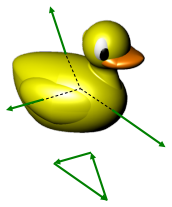
\includegraphics[width = 0.5 \textwidth]{../img/diagram38.png}
        \caption{}
    \end{figure}    
\end{minipage}
\begin{minipage}{0.45\textwidth}
    \begin{equation}
        \begin{cases}
            \begin{cases}
                \sum F_x = 0\\
                \sum F_y = 0\\
                \sum F_z = 0
            \end{cases}\\
            \begin{cases}
                \sum M_x = 0\\
                \sum M_y = 0\\
                \sum M_z = 0
            \end{cases}
        \end{cases}
    \end{equation} 
\end{minipage}
\hfill \break
These equations have to be valid for or any portion of the body.
\subsection{Stress components}
\begin{minipage}{0.4\textwidth}
    \begin{figure}[H]
        \centering
        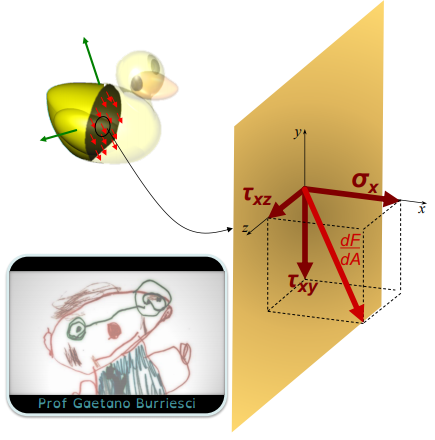
\includegraphics[width = \textwidth]{../img/diagram39.png}
        \caption{}
    \end{figure}  
\end{minipage}
\begin{minipage}{0.05\textwidth}
    \hfill
\end{minipage}
\begin{minipage}{0.55\textwidth}
    The force distribution, in a generic point of a section, will have components in the \textit{normal} and \textit{tangential} direction. 
    
    If a Cartesian reference system is fixed, with the $x$ direction normal to the section, the normal and shear stresses can be expressed in the coordinate system. 
    
    The stress can be decomposed into \textit{normal component} $\sigma_x$; and two \textit{shear components} $\tau_{xy}$ and $\tau_{xz}$.
\end{minipage}
\begin{figure}[H]
    \begin{minipage}{0.5\textwidth}
        \centering
        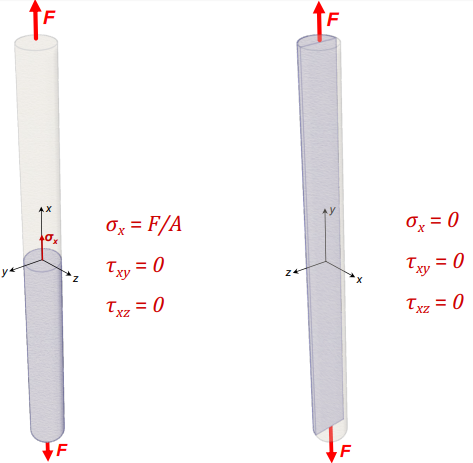
\includegraphics[height = 5cm]{../img/diagram40.png}
    \end{minipage}
    \begin{minipage}{0.5\textwidth}
        \centering
        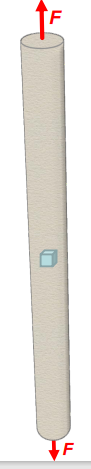
\includegraphics[height = 5cm]{../img/diagram41.png}
    \end{minipage}
    \caption{}
\end{figure}
Stress components associated with a specific direction are not sufficient to describe the stress state at one point, as they depend on the selected reference system. To define the stress state at one point, we need to consider all surfaces surrounding the point. 
\begin{figure}[H]
    \centering
    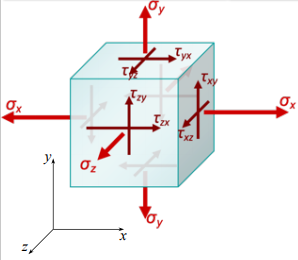
\includegraphics[height = 5cm]{../img/diagram42.png}
    \caption{}
\end{figure}
Extract from the body an infinitesimal element, sectioned along the defined Cartesian planes, of dimensions $\dif x$, $\dif y$, $\dif z$. The \textit{stress state} of the point where the element is extracted can be described by the 18 stress components (3 per each face):
\begin{align}
    \sigma = \begin{bmatrix}
        \sigma_x & \tau_{xy} & \tau_{xz}\\
        \tau_{yx} & \sigma_y & \tau_{yz}\\
        \tau_{zx} & \tau_{zy} & \sigma_z
    \end{bmatrix} \hspace{1cm}
    \begin{array}{l}
        \tau_{xy} = -\tau_{yx}\\
        \tau_{xz} = -\tau_{zx}\\
        \tau_{yz} = -\tau_{zy}
    \end{array}
\end{align}
Equilibrium of forces and moments reduces the independent components to six. The complete \textit{state of stresses} at a point is defined by the six stress components:
\begin{equation}
    \sigma_x, \, \sigma_y, \, \sigma_z; \, \tau_{xy}, \, \tau_{yz}, \, \tau_{zx}
\end{equation}
\subsubsection{Bidimensional case}
\begin{figure}[H]
    \centering
    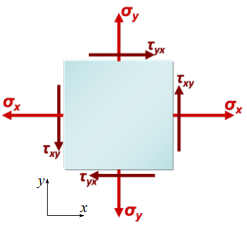
\includegraphics[height = 5cm]{../img/diagram43.png}
    \caption{}
\end{figure}
In the common cases of plane state of stress (all stress components lay on a plane), the entire state of stress can be defined by only three stress components:
\begin{equation}
    \sigma_x, \, \sigma_y; \, \tau_{xy} \hspace{1cm} \sigma = \begin{bmatrix}
        \sigma_x & \tau_{xy}\\
        \tau_{yx} & \sigma_y
    \end{bmatrix}
\end{equation}
\subsection{Normal and shear stress in a plane $\sigma$ \& $\tau @ \theta$}
\begin{figure}[H]
    \centering
    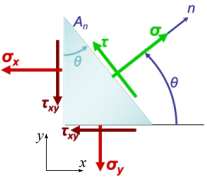
\includegraphics[height = 5cm]{../img/diagram44.png}
    \caption{}
\end{figure}
Imagine to cut the infinitesimal element with a a plane parallel to $z$, with normal $n$ at an arbitrary angle $\theta$ from $x$. Due to equilibrium, the new section of area $A_n$ will be characterised by normal and shear stresses $\sigma$ and $\tau$. 
\subsubsection{Normal component of the stress (equilibrium along $n$)}
\begin{align}
    &\sigma \cdot A_n\\
    &-\sigma_x \left(A_n \cos \theta\right)\cos\theta - \tau_{xy} \left(A_n\cos\theta\right)\sin\theta\\
    &-\sigma_y \left(A_n\sin\theta\right)\sin\theta - \tau_{xy}\left(A_n\sin\theta\right)\cos\theta\\
    &=0\\
    \sigma &= \sigma_x \cos^2 \theta + \sigma_y \sin^2 \theta + 2\tau_{xy} \sin\theta \cdot \cos\theta
\end{align}
\subsubsection{Shear component of the stress (equilbrium along normal to $n$ in the plane)}
\begin{align}
    &\tau \cdot A_n\\
    &+\sigma_x \left(A_n\cos\theta\right)\sin\theta - \tau_{xy}\left(A_n\cos\theta\right)\cos\theta\\
    &-\sigma_y \left(A_n\sin\theta\right)\cos\theta + \tau_{xy}\left(A_n\sin\theta\right)\sin\theta\sin\theta\\
    &=0\\
    \tau &= - \left(\sigma_x - \sigma_y\right)\sin\theta \cdot \cos\theta + \tau_{xy}\left(\cos^2\theta-\sin^2\theta\right)
\end{align}
\subsubsection{Normal and shear component of the stress}
Since:
\begin{align}
    \cos^2 \theta &= \frac{1}{2} \left(1 + \cos 2\theta\right)\\
    \sin^2 \theta &= \frac{1}{2} \left(1 - \cos 2\theta\right)\\
    \sin\theta \cdot \cos\theta &= \frac{1}{2}\sin 2\theta
\end{align}
Expressions of $\sigma$ and $\tau$ become:
\begin{align}
    \sigma &= \frac{1}{2} \sigma_x \left(1+\cos 2\theta \right) + \frac{1}{2}\sigma_y\left(1-\cos 2\theta\right) + \tau_{xy} \sin 2\theta\\
    \tau &= - \left(\sigma_x - \sigma_y\right) \left(\frac{1}{2}\sin 2\theta\right) + \frac{1}{2}\tau_{xy} \left[\left(1+\cos 2\theta\right)-\left(1-\cos 2\theta\right)\right]
\end{align}
Further simplification:
\begin{align}
    \sigma &= \frac{\sigma_x + \sigma_y}{2} + \frac{\sigma_x - \sigma_y}{2}\cos 2\theta + \tau_{xy}\sin 2\theta\\
    \tau &= - \frac{\sigma_x - \sigma_y}{2}\sin 2\theta + \tau_{xy}\cos 2\theta
\end{align}
Given a specific state of stress, at a point $P$, these expressions give the normal and tangential stress to any plane passing through the point.
\section{Principal stress}
\subsection{Maximum and minimum stress}
$\sigma$ and $\tau$ vary as the selected plane changes inclination. The maximum and minimum of $\sigma$ when: 
\begin{gather}
    \frac{\dif \sigma}{\dif \theta} = 0 \rightarrow \frac{\dif \sigma}{\dif \theta} = - \left(\sigma_x - \sigma_y\right)\sin 2\theta + 2\tau_{xy}\cos 2\theta = 0\\
    \tan 2\theta = \frac{2\tau_{xy}}{\sigma_x - \sigma_y}
\end{gather}
The function $\tan 2\theta$ defines 2 orientations in the range 0-\SI{360}{\degree} with \SI{90}{\degree} inclination with respect to each other. The max and min normal stresses are called \textbf{principal stresses} (respectively $\sigma_1$ and $\sigma_2$) and their planes \textbf{principal planes}. The minimum of the tangential shear stresses are zero on the \textbf{principal planes}.
\begin{figure}[H]
    \centering
    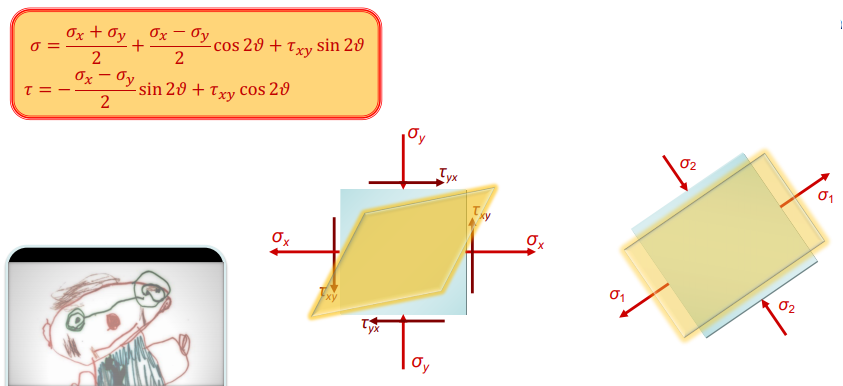
\includegraphics[width = 0.9\textwidth]{../img/diagram45.png}
    \caption{}
\end{figure}
\section{Mohr's circles}
\begin{figure}[H]
    \centering
    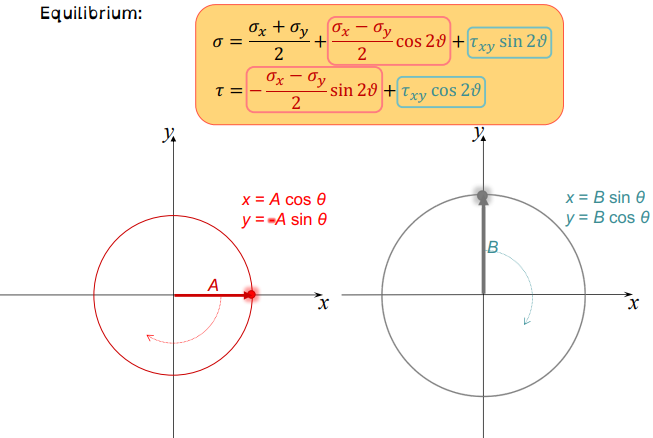
\includegraphics[height = 0.3 \textheight]{../img/diagram46.png}
    \caption{}
\end{figure}
\begin{figure}[H]
    \centering
    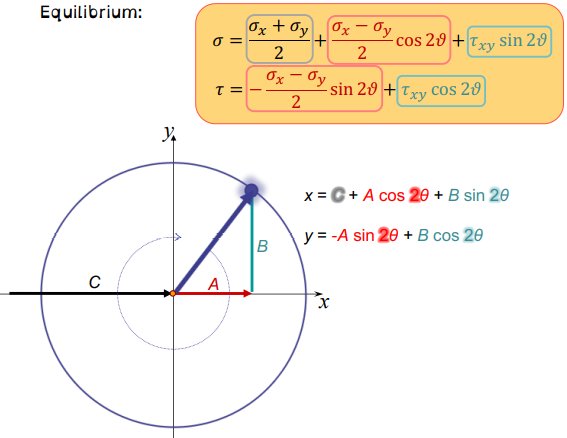
\includegraphics[height = 0.3 \textheight]{../img/diagram47.png}
    \caption{}
\end{figure}
\begin{figure}[H]
    \centering
    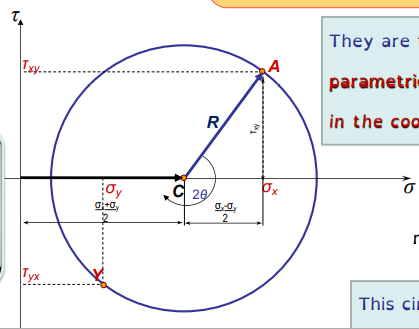
\includegraphics[height = 0.2 \textheight]{../img/diagram48.png}
    \caption{}
\end{figure}
Mohr's circles are the equations of a circle in parametric form (with parameter $\theta$, in the coordinates $\sigma$ and $\tau$).
\begin{gather}
    \textrm{centre: } C \equiv \left(\frac{\sigma_x + \sigma_y}{2}, \, 0\right)\\
    \textrm{radius: } R = \sqrt{\left(\frac{\sigma_x - \sigma_y}{2}\right)^2 + \tau^2_{xy}}
\end{gather}
Mohr's circles give a graphical representation of the state of stress in one point, describing the normal and tangent component of the stress for any plane passing through the point. The points on the Mohr's circles represent combinations of normal and shear stress that exist at all possible orientations. 
\begin{quotation}
    Note that angles in Mohr's circles are double angles and their direction is opposite to the physical one.
\end{quotation}
This can be fixed by inverting the $\tau$ axis.
\subsection{Construction of Mohr's circles - A}
The knowledge of the tensors, $\sigma_x$, $\sigma_y$ and $\tau_{xy}$ relative to any plane is sufficient to build the Mohr's circle:
\begin{enumerate}
    \item Plot the coordinates $\sigma_x$ and $\tau_{xy}$ (relative to position '$X$') in the $\sigma - \tau$ plane. This is along the $x$-axis and then corresponds to the angle $\theta = 2\theta = 0$.
    \item Plot the coordinates $\sigma_y$ and $\tau_{yx}$ (relative to position '$Y$') in the $\sigma - \tau$ plane. This is along the $y$-axis and corresponds to the angle $\theta = \SI{90}{\degree}$ ($2\theta = \SI{180}{\degree}$).
    \item The intersection of the line joining '$X$' and '$Y$' with $\sigma$-axis identifies the centre $C$ of the circle ($C$ has abscissa equal to the average of $\sigma_x$ and $\sigma_y$).
    \item Use '$C$' and '$X$' (or '$Y$') to build the circle.
\end{enumerate}
\begin{figure}[H]
    \begin{minipage}{0.25\textwidth}
        \centering
        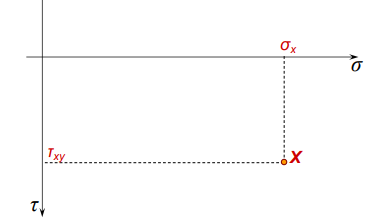
\includegraphics[width=\textwidth]{../img/diagram49.png}   
    \end{minipage}
    \begin{minipage}{0.25\textwidth}
        \centering
        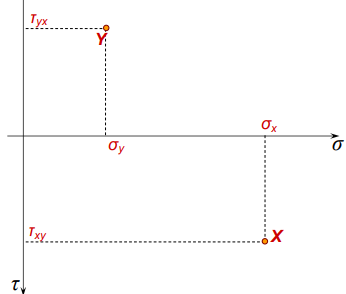
\includegraphics[width=\textwidth]{../img/diagram52.png}   
    \end{minipage}
    \begin{minipage}{0.25\textwidth}
        \centering
        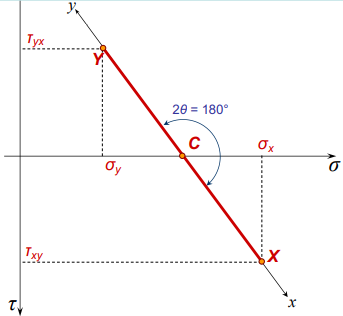
\includegraphics[width=\textwidth]{../img/diagram50.png}   
    \end{minipage}
    \begin{minipage}{0.23\textwidth}
        \centering
        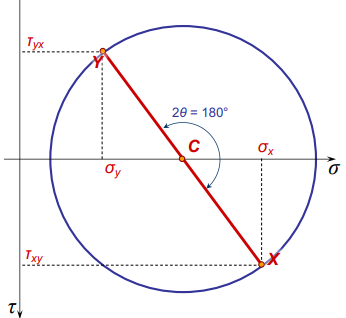
\includegraphics[width=\textwidth]{../img/diagram51.png}   
    \end{minipage}
    \caption{}
\end{figure}
\subsection{Construction of Mohr's circles - B}
The knowledge of the tensors, $\sigma_x$, $\sigma_y$ and $\tau_{xy}$ relative to any plane is sufficient to build the Mohr's circle:
\begin{enumerate}
    \item Determine the centre $C$ of the circle from: $C \equiv \left(\frac{\sigma_x + \sigma_y}{2}, \, 0\right)$.
    \item Determine the radius $R$ of the circle from: $R = \sqrt{\left(\frac{\sigma_x - \sigma_y}{2}\right)^2 + \tau^2_{xy}}$
    \item Draw a circle of centre $C$ and radius $R$.
    \item Position on the circle points relative to '$X$' (and '$Y$') to identify $x$-axis.
\end{enumerate}
\begin{figure}[H]
    \begin{minipage}{0.25\textwidth}
        \centering
        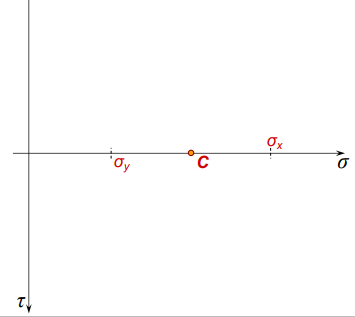
\includegraphics[width=\textwidth]{../img/diagram53.png}   
    \end{minipage}
    \begin{minipage}{0.25\textwidth}
        \centering
        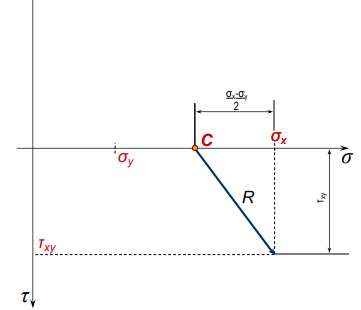
\includegraphics[width=\textwidth]{../img/diagram54.png}   
    \end{minipage}
    \begin{minipage}{0.25\textwidth}
        \centering
        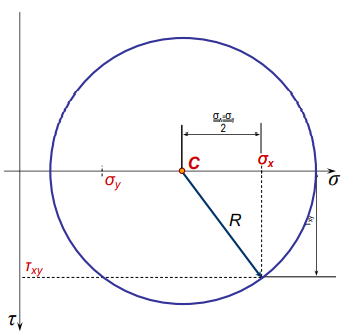
\includegraphics[width=\textwidth]{../img/diagram55.png}   
    \end{minipage}
    \begin{minipage}{0.25\textwidth}
        \centering
        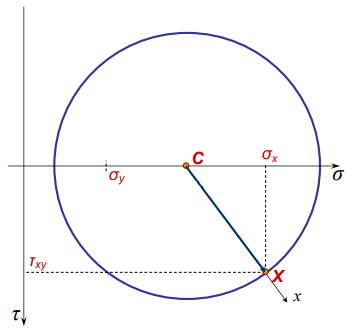
\includegraphics[width=\textwidth]{../img/diagram56.png}   
    \end{minipage}
    \caption{}
\end{figure}
\section{Application of Mohr's circles}
\subsection{Determination of principal stresses}
The most important application of Mohr's circles is the geometrical determination of the value and direction of the principal stress. 
\begin{figure}[H]
    \centering
    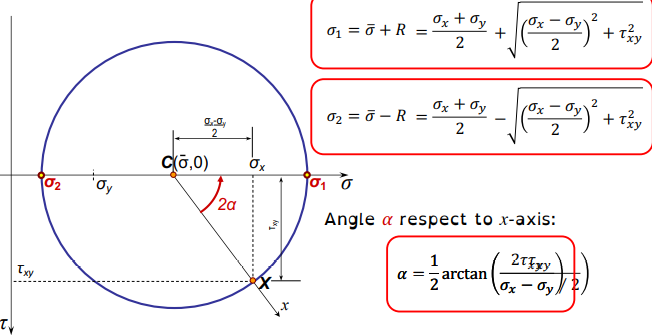
\includegraphics[height = 6cm]{../img/diagram57.png}
    \caption{}
\end{figure}
\subsection{Determination of max shear stress}
Another Mohr's circle application is the geometrical determination of the value and direction of the maximum shear stresses.
\begin{figure}
    \begin{minipage}{0.49\textwidth}
        \begin{figure}[H]
            \centering
            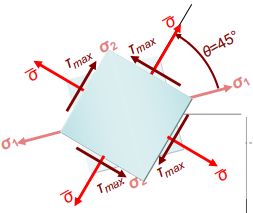
\includegraphics[width = \textwidth]{../img/diagram59.png}
        \end{figure}
    \end{minipage}
    \begin{minipage}{0.5\textwidth}
        \begin{figure}[H]
            \centering
            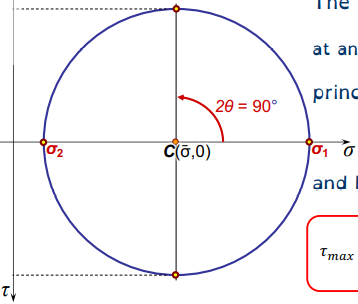
\includegraphics[width = \textwidth]{../img/diagram58.png}
        \end{figure}
    \end{minipage}
    \caption{}
\end{figure}
The \textit{maximum shear stress} is always at an angle $\theta = \SI{45}{\degree} \, (2\theta=\SI{90}{\degree})$ with the principal stress directions and has magnitude equal to:
\begin{equation}
    \tau_{max} = R = \sqrt{\left(\frac{\sigma_x - \sigma_y}{2}\right)^2 + \tau^2_{xy}} = \frac{\sigma_1-\sigma_2}{2}
\end{equation}
Mohr's circles allow to calculate the stress tensors for any plane.
\begin{figure}
    \begin{minipage}{0.49\textwidth}
        \begin{figure}[H]
            \centering
            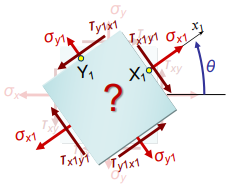
\includegraphics[width = \textwidth]{../img/diagram60.png}
        \end{figure}
    \end{minipage}
    \begin{minipage}{0.5\textwidth}
        \begin{figure}[H]
            \centering
            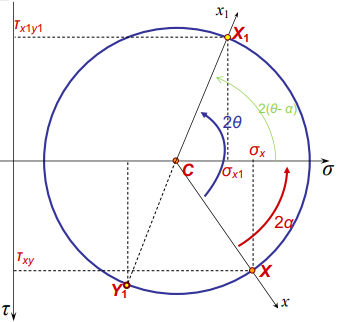
\includegraphics[width = \textwidth]{../img/diagram61.png}
        \end{figure}
    \end{minipage}
    \caption{}
\end{figure}
\begin{align}
    \sigma_{x1} &= \bar{\sigma} + R\cos 2(\theta - \alpha)\\
    \sigma_{y1} &= \bar{\sigma} - R\cos 2(\theta - \alpha)\\
    \tau_{x1 \, y1} &= -R \sin 2(\theta - \alpha)
\end{align}
With $\bar{\sigma} = \frac{\sigma_x + \sigma_y}{2} = \frac{\sigma_1 + \sigma_2}{2}$ and $R = \sqrt{\left(\frac{\sigma_x - \sigma_y}{2}\right)^2 + \tau^2_{xy}} = \frac{\sigma_1-\sigma_2}{2}$.
\section{Tri-axial state of stress}
\subsection{Plane stress state}
We have seen that if we only consider two stresses in the plane, the state of stress is defined by 3 stress components (tensors).
\begin{figure}[H]
    \centering
    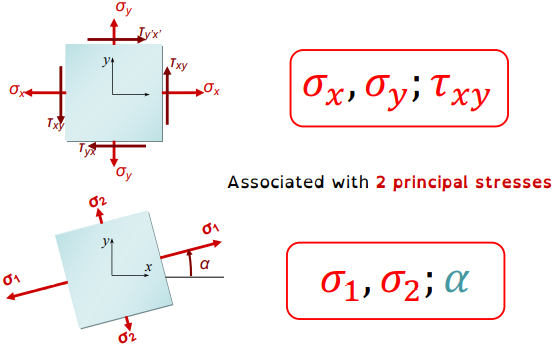
\includegraphics[height = 5cm]{../img/diagram62.png}
    \caption{}
\end{figure}
\subsection{Tri-axial stress state}
In the most generic state of stress (tri-axial) is defined by 6 stress components (tensors): 
\begin{figure}[H]
    \centering
    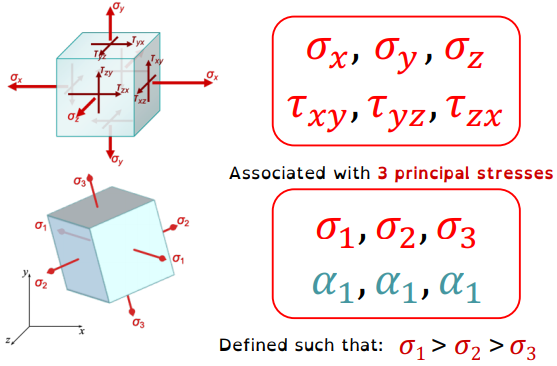
\includegraphics[height = 5cm]{../img/diagram63.png}
    \caption{}
\end{figure}
\subsection{Complete Mohr's circles}
Mohr's representation will be characterised by 3 circles, relative to the three orthogonal principal planes: 
\begin{figure}[H]
    \centering
    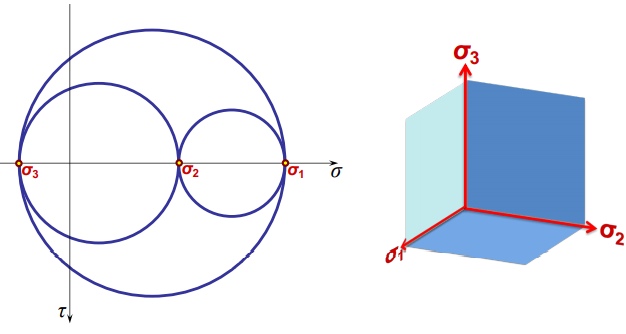
\includegraphics[height = 5cm]{../img/diagram64.png}
    \caption{}
\end{figure}
Maximum shear stresses in the three principal planes will be:
\begin{equation}
    (\tau_{max})_3 = \frac{|\sigma_1 - \sigma_2|}{2} \hspace{1cm} (\tau_{max})_1 = \frac{|\sigma_2 - \sigma_3 |}{2} \hspace{1cm} (\tau_{max})_2 = \frac{|\sigma_3 - \sigma_1 |}{2}
\end{equation}
Absolute maximum equal to the largest value.
\begin{equation}
    \tau_{max} = (\tau_{max})_2 = \frac{\sigma_1 - \sigma_3}{2}
\end{equation}
\begin{figure}[H]
    \centering
    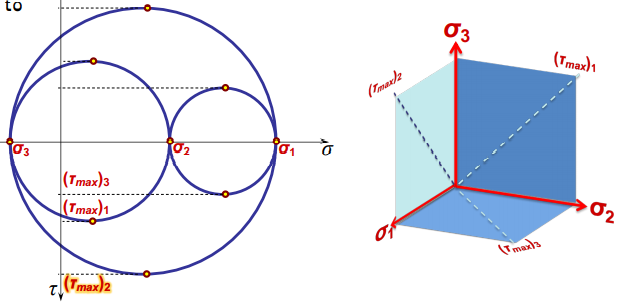
\includegraphics[height = 5cm]{../img/diagram65.png}
    \caption{}
\end{figure}
Also a plane state of stress ($\sigma_1 \neq 0, \, \sigma_2 \neq 0, \, \sigma_3 = 0$) is associated with three Mohr's circles. The maximum shear stress is not necessarily in the plane of the stresses that are different from zero!
\begin{figure}[H]
    \centering
    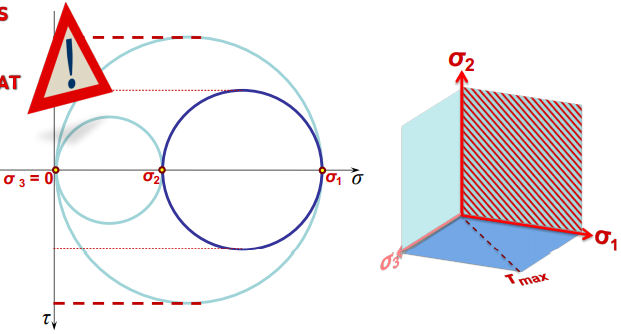
\includegraphics[height = 5cm]{../img/diagram66.png}
    \caption{}
\end{figure}
\section{Stress strain relations}
\subsection{Principal strains}
In the case of an isotropic, linear-elastic material, the \textit{principal strains} are defined as the strains in the directions of the principal stresses.
\begin{equation}
    \varepsilon_1, \, \varepsilon_2, \, \varepsilon_3
\end{equation}
Principal stress and principal strains are linked through the Young's Modulus and the Poisson ratio (constitutive relations).
\subsection{What is the Poisson's ratio? ($\nu$)}
The Poisson's Ratio is the negative ratio of the transverse to longitudinal strain:
\begin{equation}
    \nu = -\frac{\textrm{transverse strain}}{\textrm{longitudinal strain}} = - \frac{\varepsilon_t}{\varepsilon_l}
\end{equation}
\begin{figure}[H]
    \centering
    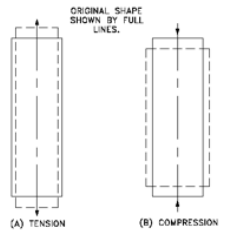
\includegraphics[height = 5cm]{../img/diagram67.png}
    \caption{}
\end{figure}
\subsection{Uni-axial case}
\begin{equation}
    \begin{array}{l}
        \varepsilon_1 = \frac{\sigma_1}{E}\\
        \varepsilon_2 =-\frac{\nu}{E}\sigma_1\\
        \varepsilon_3 =-\frac{\nu}{E}\sigma_1    
    \end{array} \hspace{1cm} \begin{array}{l}
        \sigma_1 = E\varepsilon_1\\
        \sigma_2 = 0\\
        \sigma_3 = 0
    \end{array}
\end{equation}
\begin{figure}[H]
    \centering
    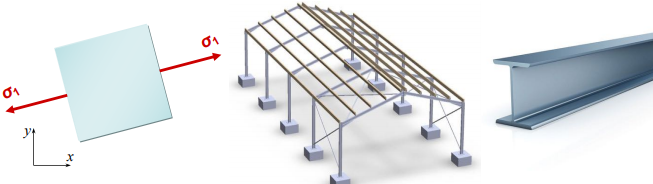
\includegraphics[width = 0.8\textwidth]{../img/diagram68.png}
    \caption{}
\end{figure}
\subsection{Bi-axial case}
\begin{equation}
    \begin{array}{l}
        \varepsilon_1 = \frac{1}{E}\left[\sigma_1-\nu\sigma_2\right]\\
        \varepsilon_2 = \frac{1}{E}\left[\sigma_2-\nu\sigma_1\right]\\
        \varepsilon_3 =-\frac{\nu}{E}\left(\sigma_1 + \sigma_2\right)    
    \end{array} \hspace{1cm} \begin{array}{l}
        \sigma_1 = \frac{E}{1-\nu^2}\left[\varepsilon_1 + \nu \varepsilon_2\right]\\
        \sigma_2 = \frac{E}{1-\nu^2}\left[\varepsilon_2 + \nu \varepsilon_1\right]\\
        \sigma_3 = 0
    \end{array}
\end{equation}
\begin{figure}[H]
    \centering
    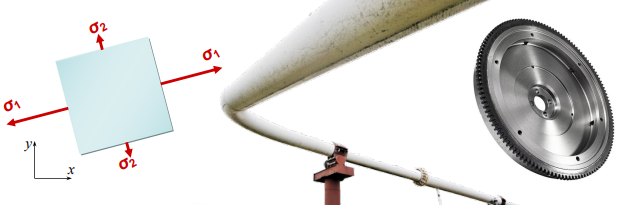
\includegraphics[width = 0.8\textwidth]{../img/diagram69.png}
    \caption{}
\end{figure}
\subsection{Tri-axial case}
\begin{equation}
    \begin{array}{l}
        \varepsilon_1 = \frac{1}{E}\left[\sigma_1-\nu\left(\sigma_2 + \sigma_3\right)\right]\\
        \varepsilon_2 = \frac{1}{E}\left[\sigma_2-\nu\left(\sigma_3 + \sigma_1\right)\right]\\
        \varepsilon_3 = \frac{1}{E}\left[\sigma_3-\nu\left(\sigma_1 + \sigma_2\right)\right]    
    \end{array} \hspace{1cm} \begin{array}{l}
        \sigma_1 = \frac{E}{\left(1+\nu\right)\left(1-2\nu\right)}\left[\left(1-\nu\right)\varepsilon_1 + \nu \left(\varepsilon_2 + \varepsilon_3\right)\right]\\
        \sigma_2 = \frac{E}{\left(1+\nu\right)\left(1-2\nu\right)}\left[\left(1-\nu\right)\varepsilon_2 + \nu \left(\varepsilon_3 + \varepsilon_1\right)\right]\\
        \sigma_3 = \frac{E}{\left(1+\nu\right)\left(1-2\nu\right)}\left[\left(1-\nu\right)\varepsilon_3 + \nu \left(\varepsilon_1 + \varepsilon_2\right)\right]
    \end{array}
\end{equation}
\begin{figure}[H]
    \centering
    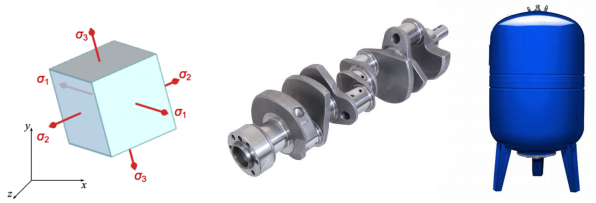
\includegraphics[width = 0.8\textwidth]{../img/diagram70.png}
    \caption{}
\end{figure}
\end{document}